% This is lnbip.tex the demonstration file of the LaTeX macro package for
% Lecture Notes in Business Information Processing from Springer-Verlag.
% It serves as a template for authors as well.
% version 1.0 for LaTeX2e
%
\documentclass[lnbip]{svmultln}
%
\usepackage{makeidx}  % allows for indexgeneration
\usepackage{graphicx}
% \makeindex          % be prepared for an author index
%
\newcommand{\mari}[1]{\footnote{MARI: #1}}
\begin{document}
%
\mainmatter              % start of the contribution
%
\title{Prototypes are forever\\
  Evolving from a prototype project\\ to a full-featured system}
%
\titlerunning{Prototypes are forever}  % abbreviated title (for running head)
%                                     also used for the TOC unless
%                                     \toctitle is used
%
\author{Hugo Corbucci\inst{1} and Mariana V. Bravo \inst{1}}
%
\authorrunning{Hugo Corbucci et al.}   % abbreviated author list (for running head)
%
%%%% list of authors for the TOC (use if author list has to be modified)
\tocauthor{Hugo Corbucci and Mariana V. Bravo}
%
\institute{Agilbits, Sao Paulo, Brazil,\\
\email{{hugo,marivb}@agilbits.com.br}}

\maketitle              % typeset the title of the contribution
% \index{Ekeland, Ivar} % entries for the author index
% \index{Temam, Roger}  % of the whole volume
% \index{Dean, Jeffrey}

\begin{abstract}        % give a summary of your paper

%TODO Abstract
This paper shows you how to handle prototype projects.
%                         please supply keywords within your abstract

%TODO Keywords
\keywords {prototype, agile methods, }
\end{abstract}
%
\section{Introduction}

Prototyping is an activity that most developers have heard about. Fred
Brooks mentioned it in The Mythical Man-Month \cite{Brooks1975} as one
of the best ways to provide a quick view of a feature to the clients
or users to help them make a choice. Dynamic System Development Method
(DSDM)\cite{DSDM} is heavily based on prototyping and other agile
methods also adopt many ideas related to it. However, those who have
had some experience with this practice feel uncomfortable with it.

Successful software prototypes look very much like complete features
given a certain execution path. Therefore it is common that the
customers get so happy with it that they want to integrate the
prototypes to the working system and move on. The problem is that
prototypes are frequently created in a ``quick and dirty'' fashion and
the result is not adequate to be incorporated in a full-featured
system. Yet it is quite hard to explain this fact to the stakeholders
who usually do not want to invest any more money in this ``already
working'' feature. The consequence is that they switch priorities and
work efforts to other parts of the system and leave the rough
prototype lost within the code base. Months or years later, the
prototype becomes a part of the system but is filled with bugs,
unhandled corner cases and, frequently, crappy code. Nobody remembers
what it was supposed to do or whether it is really
important. Maintainability gets deeply affected and developers have
that natural and unpleasant I-told-you-so feeling. %TODO trauma?

Developers that have been through the pain of maintaining those dirty
prototypes are not enthusiastic to work with prototypes anymore. If
they have to, they make it so that there will be absolutely no way to
integrate the prototype to the existing system by either using a
different platform, language or even creating prototypes in other
medias. That inflexibility can reduce the ability of responding to
changes quickly and therefore harm the clients' interests.

This paper presents how a four-people collocated team managed to start
a prototyping project and evolve it naturally to a full-featured
software. The organization of this work follows a chronological order
as the project evolved. Section \ref{sec:start} will present the
project as it was first presented to the development team. Section
\ref{sec:working} presents the work process established by the team to
create the software based on prototypes.  After some time, the team
felt that the customer was shifting to a full featured idea as
described in Section \ref{sec:changes}. The following section (Section
\ref{sec:adapting}) shows how the team adapted to those changes to
accommodate both ideas. Finally Section \ref{sec:nowadays} presents the
current status of the project and Section \ref{sec:conclusion}
concludes with a summary of practices that were useful to pass through
this experience without much pain.

\section{Starting the project}
\label{sec:start}

Back in March 2008, our company was hired to do some consulting for
one of the largest movie producing companies in Brazil. The client had
a great idea for a software to write movie scripts but had absolutely
no knowledge about software development.  He wanted to mature the idea
and understand how much investment it would take to turn it into
working software in order to establish his business plan. The
company's job at the time was to scout the market, discover
competitors and provide an estimation of the work needed to develop
the client's idea.

For such work, one consultant was assigned to understand what were the
client's needs and desires and two developers were asked to analyze
the existing script writing programs and evaluate the possible
development paths. After about 3 weeks of consulting and studies, the
team handed a deck full of story cards with two estimates each, based
on the use of two possible platforms. The first platform was an
existing open source software with several features and a copy-left
license. The second one was an Eclipse Rich Client Application
developed from scratch using Eclipse's open source framework.

This initial estimation suggested that a four people team with a
half-time dedication would be able to build a working prototype of
each feature described in about nine months of development using the
existing open source software and about one year using Eclipse's
platform. The open source solution had the advantage to provide full
functionality of several other features. For a complete system, the
estimation was well over 2 years of work on the Eclipse version and
about a year and a half for the open source one.

After some discussion, the client opted for the Eclipse based solution
due to the license restriction of the open source one which conflicted
with his business plan. He also chose to develop only a prototype of
the idea since 2 years seemed like a too heavy investment for him
alone.

After the investigation phase, the consulting contract ended and a new
one with a majority of development time was established. Originally,
this new contract mentioned a 4 developers team working on an open
scope providing 160 hours of work each month. It specifically stated
that the developers would work on pairs all the time and that the
developed system should have automated tests to the production code.

The project goal was to create a software prototype with most faked or
simplified features and a few working ones. The client would use this
prototype to present his ideas to investors by October 2008. This
meeting would either boost the project's development to a full
featured system if the investors liked the idea or end its development
in case they rejected it.

That was the team's vision of the project when the development
begun. A short seven months project whose fate would be decided by its
capacity to impress investors. Therefore, the main goal was to provide
an excellent support for the client's demonstration to ensure the
project's growth and success. The next section (Section
\ref{sec:working}) describes how the team organized itself to achieve
this goal.

\section{Developing a work process}\mari{Sugestoes pro nome da secao: Working with prototypes,Developing prototypes,Prototyping phase - vc nem fala muito do nosso work process}
\label{sec:working}

Given the project's situation\mari{acho que situation nao eh a palavra aqui. que tal goal? objective? purpose?}, the customer was always pushing for new features as fast as possible considering only one specific usage scenario. This meant that, for most features, there were several cases which the team was asked \textbf{not} to handle. Regarding the source code, this meant a lot of conditionals\mari{nao sei se tinha a lot of conditionals... acho que estava mais pra assumir que so tinha um caso possivel, a gente nao verificava se estava no caso...}, several spikes becoming permanent solutions and a fair amount of unhandled exceptions, ignored errors or non functional regular behaviors\mari{nao entendi o que vc quer dizer por "non functional regular behaviors". a frase parece nao fazer nenhum sentido...}.

The team knew since the beginning that the client would change his mind over time. After all, it was partly to better understand his idea and its applicability that he wanted to build this prototype. So things\mari{things parece meio generico. o que mudaria? requirements? priorities? features?} were going to change and features would be developed to later be thrown away while code produced only for a quick spike was going to become part of the system. Therefore, since the beginning the team invested a little on design, automated tests and refactoring and made it clear for the client that there would be some work done on features after he accepted them in order to polish the work.\mari{Uma alternativa, pq nao gosto muito desse little: Therefore, since the beginning the team invested on design, automated tests and refactoring, even if just enough to keep the system flexible to receive the next changes. The team also made it clear for the client that there would be some work done on features after he accepted them in order to polish the work.}

The first few iterations went quite smooth. The main features developed involved importing a script in a text-only format, providing a simple text marking feature and a feature to manipulate and visualize these marks. For those features, it was quite simple to avoid gaps\mari{o que eh gaps? nao entendi a frase} since there were not many business rules involved. Problems started to appear once the script writing business rules started to show up\mari{que problems? essa frase parece meio solta... sera que eh pq eu nao entendi a frase anterior?}.

The client's demonstration\mari{posso colocar so "demo script"?} script was evolving as the software did and the team soon started to add conditionals to ignore cases he would not enter in. By October 2008, the main features\mari{to sentindo falta de um paragrafo "classificando" as features que tinhamos no inicio, estilo o spreadsheet que o paulo mandou pra gente laaaa no inicio do projeto (ver email "Fwd: Story Touch projeto" do Ale) - vamos conversar} were ready\mari{ready for the demonstration, but not "done-done", they were prototyped.} but new discovered features were still incipient\mari{quais features sao essas? na verdade a gente estava comecando a entrar no editor, so que isso nao era novo, ja tinha desde o comeco} and the client was not feeling confident to present the software to the investors. However, he started to make contact with a few people to schedule a meeting by the end of November 2008 or start of December 2008. Those dates became our new deadline until which all efforts should be focused on making those incipient features available for the demonstration.

At this point, the pressure for new features increased since the project's fate would be decided at the demonstration and it was close! The customer wanted the team to ignore corner cases, speed up delivery and ensure the demonstration would run smoothly. The excitement from the important presentation to other people (only our one client and us had seen the software so far) was a strong motivation for the development team to deliver all features the client had asked for. Yet, despite unit testing and pair programming being mandatory rules on the team, the general will to quickly deliver the features decreased the code quality.

Things were getting quite unpleasant from a development perspective but since the client satisfaction was still high, there was little that could be done. However, external interference was about to change a bit the situation. Section \ref{sec:changes} will explain how the project got affected and what new direction those changes pointed to.

\section{Changing the rules}
\label{sec:changes}

December 2008 arrived and passed without any meeting. The company that
the client was in contact with had just been acquired by another one
so any project presentation was useless until things settled
down. That news pushed the deadline away for another 3 or 4 months at
least. By February 2010 came the information that the client had
formed a dramaturgy experts group to help him understand better how to
structure the software.

This new context relieved a 4 months pressure of upcoming deadline
over a team which was beginning to feel the burden of unhandled
technical debt. All members of the development team agreed that the
code was getting complex and the quality was decreasing which was
affecting productivity and speed. The software was now going to have a
set of beta testers and it needed to perform decently to allow the
users to suggest improvements in the work system.

The general feeling was that the project was no longer aimed at a
simple presentation to investors. It was softly switching to a more
elaborate and end user oriented software. The current development
approach would not be able to support this new use of the system. The
change had to be clear to the client so that development efforts would
be directed to address this new way of working.

The warnings came quickly from the dramaturgy study group. They
started having troubles with several known and unknown corner cases,
behaviors and just plain old bugs. The client started to notice that
the users were having several troubles with the software and decided
we needed to invest more in usability and user experience. To which
the team replied that it would also mean less new features.

At this point, the client started to understand the dilemma that the
developers had felt so far. How to keep a good rhythm of new features
and still cover most use cases of existing features? Another critical
issue in the software was that, so far, most features aimed at
visualization and insertion of meta data in the movie script but users
were claiming for basic text editing features ignored so far.

The team estimated that to have an editor with the basic features
expected by the client would take at least three full iterations. This
was completely unacceptable to the client since it would mean no new
feature until the moment when he would possibly be able to show the
software to investors. So he took another action which indicated
changes in the business plan of the project. He decided he wanted to
have another team working on an editor feature that would allow all
the features he wanted.

The team did some research and ended up discovering an open source
Eclipse Rich Client WYSIWYG (What You See Is What You Get) HTML
editor\footnote{\url{http://onpositive.com/richtext/} - Last accessed
  on 20/02/2010}. The editor relied on a reimplementation of Eclipse's
StyledText component which is responsible for rendering text within
Eclipse editors. This kind of knowledge was close enough from the one
needed to implement the features our client wanted on our
application. So the client outsourced the development of this
underlying infra-structure as a way to keep the feature producing
speed while attending the users' requests.

It took about two iterations to establish the new rhythm and adapt to
the idea of a new work process. After that, the development team was
concerned with the increasing complexity so they started to track some
data from the source code. The first metrics was the amount of
\texttt{FIXME}, \texttt{TODO} and \texttt{XXX} marks in the code. As
previously mentioned, the development team added those marks
everywhere the felt a corner case or a behavior existed but was not
handled. Each mark had a small comment associated and the kind of the
mark determined the criticality of the problem. Figure \ref{fig:TODOs}
shows the evolution of those marks during the project.

\begin{figure}[hbt]
  \centerline{
    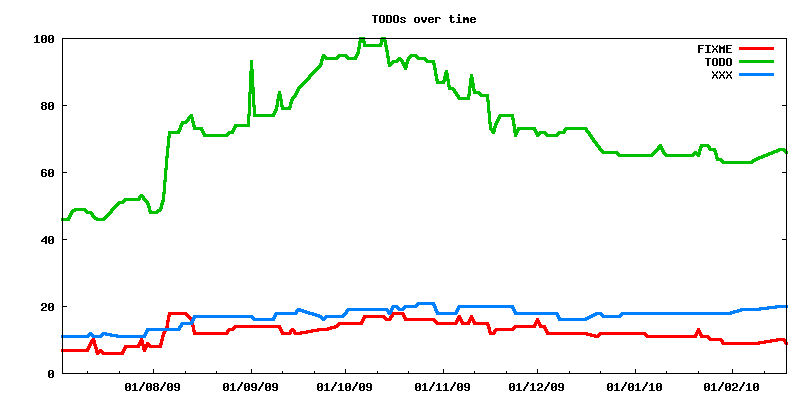
\includegraphics[width=120mm]{TODOs.png}
  }
  \caption{Evolution of FIXME, TODO and XXX marks in the source code}
  \label{fig:TODOs}
\end{figure}

\begin{figure}[hbt]
  \centerline{
    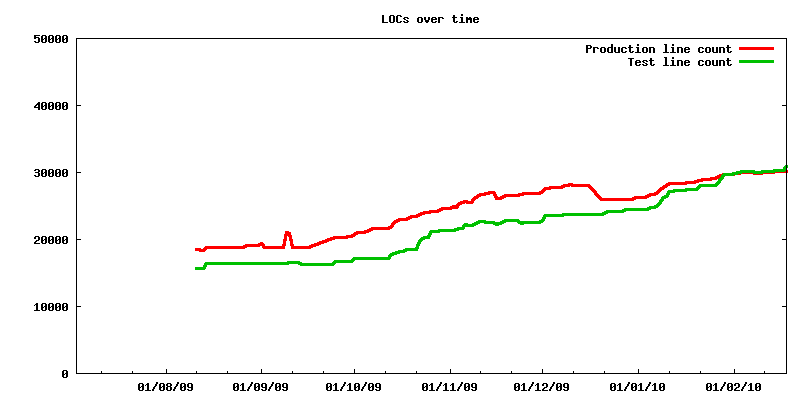
\includegraphics[width=120mm]{LOCs.png}
  }
  \caption{Evolution of production }
  \label{fig:LOCs}
\end{figure}

\begin{figure}[hbt]
  \centerline{
    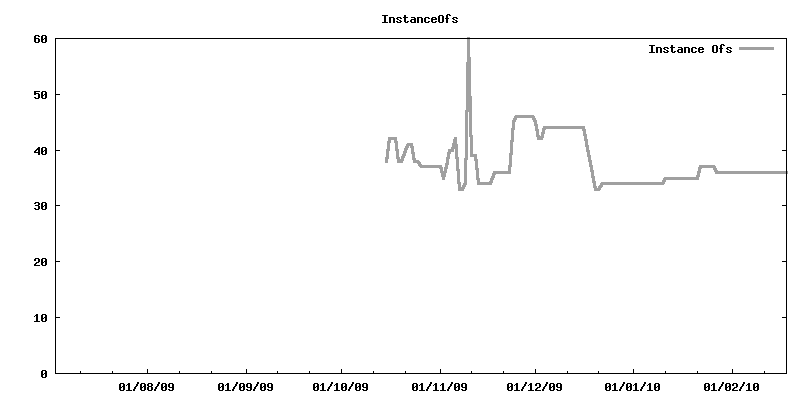
\includegraphics[width=120mm]{InstanceOfs.png}
  }
  \caption{Evolution of instanceof in the code }
  \label{fig:InstanceOfs}
\end{figure}

\begin{figure}[hbt]
  \centerline{
    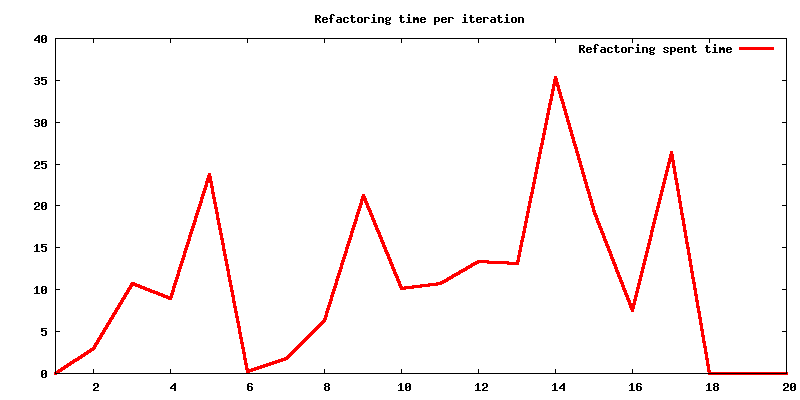
\includegraphics[width=120mm]{refactoring.png}
  }
  \caption{Explicit refactoring time by iteration}
  \label{fig:refactoring}
\end{figure}

\section{Adapting to the new rules}
\label{sec:adapting}

Investing in reducing instanceof uses, TODOs and FIXMEs as well as
increasing line of tests. Noticing most issues are coming from
UI. SWTBot?

Effort dedication to integrate the new outsourced component developed.

Always handle (even if it means throwing an error to the log) corners
cases or unexpected input/paths. Always refactor before completing any
task. Tolerance 0 to bugs. Bug means highest priority.

Introducing another developer in the team.

\section{Current status}
\label{sec:nowadays}

Test coverage

Testing in other platforms

Merciless decoupling

\section{Conclusion}
\label{sec:conclusion}

Team's effort to keep tests level (ignoring known issues not solved).

Refactor tests.

Refactor prototypes (their code must be good).



%
% ---- Bibliography ----
%
\begin{thebibliography}{5}

\bibitem{Brooks1975} Brooks Jr., F.P.: The Mythical Man Month: Essays
  on Software Engineering. Addison-Wesley (1975)

\bibitem{DSDM} DSDM Consortium: DSDM: Business Focused Development. Addison-Wesley (2002)

\end{thebibliography}
%
\end{document}
